\documentclass{article}

\usepackage{tikz}
\usepackage{pgfplots}
\pgfplotsset{compat=newest}
\usepgfplotslibrary{patchplots}

\pagestyle{empty}


%Common symbols
%Common math symbols

%Real Numbers
	\newcommand{\Real}{\mathbb{R}}
% Kinematic Configurations
	\newcommand{\Conf}{\mathrm{C}}
% Atlas
	\newcommand{\Atlas}{\mathcal{A}}

%Lagrangiana
	\newcommand{\Lagrangian}{\mathcal{L}}

%Solutions Space
	\newcommand{\Sol}{\mathrm{Sol}}


%Funzione 3D
\pgfmathdeclarefunction{F}{2}{\pgfmathparse{100+5*(#1-5)^2+5*(#2-2)^2}}

\begin{document}
%\/\/\/\/\/\/\/\/\/\/\/\/\/\/\/\/\/\/\/\/\/\/\/\/\/\/\/\/\/\/\/\/\/\/\/\/\/\/\/\/\/\/\/\/\/\/\/\/\/\/\/\/\/\/\/\/\/\/\/\/\/\/\/\/\/\/
\section{Figura 0}
La rappresentazione 2D dello spazio delle configurazioni Cinematiche\\
\begin{tikzpicture}
\begin{axis}[axis lines=none,clip=false]

	% Il riquadro di \Conf
	\addplot[color=black] coordinates {
		(8,6) (0,6) (0,0)(8,0)(8,6)
		}node [pos=1,pin={0:$\Conf$},inner sep=0pt] {};

	% la retta di \Sol
	\addplot[color=red] coordinates {
		(0,2)
		(8,2)
	}node [pos=1,pin={0:$\Sol$},inner sep=0pt] {};
	
	% Zero section
	\node[label={270:{$0$}},circle,fill,inner sep=1pt] at (axis cs:1.25,2) {};
	% Fixed Solution
	\node[label={270:{$\phi_0$}},circle,fill,inner sep=1pt] at (axis cs:5,2) {};

	% La curva di \Sol_\epsilon
	\addplot[color=gray,smooth] coordinates {
	(6,6) (3.5,4.5)(6,3)
	(5,2) (6,1)
	(3.5,0) 
	}node [pos=1,pin={270:$\phi_\epsilon$},inner sep=0pt] {};


\end{axis}
\end{tikzpicture}



%\/\/\/\/\/\/\/\/\/\/\/\/\/\/\/\/\/\/\/\/\/\/\/\/\/\/\/\/\/\/\/\/\/\/\/\/\/\/\/\/\/\/\/\/\/\/\/\/\/\/\/\/\/\/\/\/\/\/\/\/\/\/\/\/\/\/
\section{Figura 1}
 Le variazioni di Peierels\\
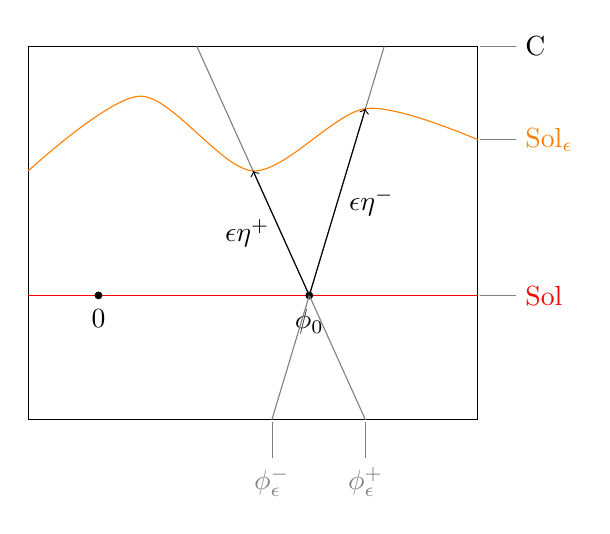
\begin{tikzpicture}
\begin{axis}[axis lines=none,clip=false]

	% Il riquadro di \Conf
	\addplot[color=black] coordinates {
		(8,6) (0,6) (0,0)(8,0)(8,6)
		}node [pos=1,pin={0:$\Conf$},inner sep=0pt] {};

	% la retta di \Sol
	\addplot[color=red] coordinates {
		(0,2)
		(8,2)
	}node [pos=1,pin={0:$\Sol$},inner sep=0pt] {};
	
	% Zero section
	\node[label={270:{$0$}},circle,fill,inner sep=1pt] at (axis cs:1.25,2) {};
	% Fixed Solution
	\node[label={270:{$\phi_0$}},circle,fill,inner sep=1pt] at (axis cs:5,2) {};

	% La curva di \Sol_\epsilon
	\addplot[color=orange,smooth] coordinates {
	(0,4) (2,5.2)(4,4)(6,5)(8,4.5)
	}node [pos=1,pin={0:$\Sol_\epsilon$},inner sep=0pt] {};

	%Variation
	\addplot[color=gray] coordinates {
		(3,6)
		(6,0)
	}node [pos=1,pin={270:$\phi_\epsilon^+$},inner sep=0pt] {};
	\addplot[color=gray] coordinates {
		(6.33333,6)
		(4.33333,0)
	}node [pos=1,pin={270:$\phi_\epsilon^-$},inner sep=0pt] {};
	
	%Perturbation
	\addplot[->] coordinates
           {(5,2) (4,4)}node [pos=0.5,label={180:$\epsilon \eta^+$},inner sep=0pt] {};
	\addplot[->] coordinates
           {(5,2) (6,5)}node [pos=0.5,label={0:$\epsilon \eta^-$},inner sep=0pt] {};


\end{axis}
\end{tikzpicture}


%\/\/\/\/\/\/\/\/\/\/\/\/\/\/\/\/\/\/\/\/\/\/\/\/\/\/\/\/\/\/\/\/\/\/\/\/\/\/\/\/\/\/\/\/\/\/\/\/\/\/\/\/\/\/\/\/\/\/\/\/\/\/\/\/\/\/
\section{Figura 2}
Rappresentazione di funzionali e di effetto\\
\begin{tikzpicture}
\begin{axis}[axis lines=none,clip=false]

	%Funzionale sulle configurazioni
	\addplot3[ mesh, color=gray,domain=0:8,y domain=0:6]
	{F(x,y)};

	% Il riquadro di \Conf
	\addplot3[color=black] coordinates {
		(8,6,0) (0,6,0) (0,0,0)(8,0,0)(8,6,0)
		}node [pos=1,pin={270:$\Conf$},inner sep=0pt] {};

	% starting value
	\node[label={270:{$\phi_0$}},circle,fill,inner sep=1pt] at (axis cs:5,2,100 ) {};

	% Curve parametrizzate sulla superficie
		\addplot3[red,domain=0:1,variable=\t,samples y=0] ({3+3*t},{6-6*t},{F(3+3*t,6-6*t)});
		\addplot3[red,domain=0:1,variable=\t,samples y=0] ({6.33333-2*t},{6-6*t},{F(6.33333-2*t,6-6*t)});


	%\\\\\\\\\\\\\\Parte 2d)\\\\\\\\\\\\\\
	% la retta di \Sol
	\addplot[color=red] coordinates {
		(0,2)
		(8,2)
	}node [pos=1,pin={270:$\Sol$},inner sep=0pt] {};
	
	% Zero section
	\node[label={270:{$0$}},circle,fill,inner sep=1pt] at (axis cs:1.25,2) {};
	
	% Fixed Solution
	\node[label={270:{$\phi_0$}},circle,fill,inner sep=1pt] at (axis cs:5,2) {};

	% La curva di \Sol_\epsilon
	\addplot[color=orange,smooth] coordinates {
	(0,4) (2,5.2)(4,4)(6,5)(8,4.5)
	}node [pos=1,pin={270:$\Sol_\epsilon$},inner sep=0pt] {};

	%Variation
	\addplot[color=gray] coordinates {
		(3,6)
		(6,0)
	}node [pos=1,pin={270:$\phi_\epsilon^+$},inner sep=0pt] {};
	\addplot[color=gray] coordinates {
		(6.33333,6)
		(4.33333,0)
	}node [pos=1,pin={270:$\phi_\epsilon^-$},inner sep=0pt] {};
	
	%Perturbation
	\addplot[->] coordinates
           {(5,2) (4,4)}node [pos=0.5,label={180:$\epsilon \eta^+$},inner sep=0pt] {};
	\addplot[->] coordinates
           {(5,2) (6,5)}node [pos=0.5,label={0:$\epsilon \eta^-$},inner sep=0pt] {};


\end{axis}
\end{tikzpicture}



%\/\/\/\/\/\/\/\/\/\/\/\/\/\/\/\/\/\/\/\/\/\/\/\/\/\/\/\/\/\/\/\/\/\/\/\/\/\/\/\/\/\/\/\/\/\/\/\/\/\/\/\/\/\/\/\/\/\/\/\/\/\/\/\/\/\/
\section{Figura 3}
 Il Caso dei funzionali lagrangiani semplici\\
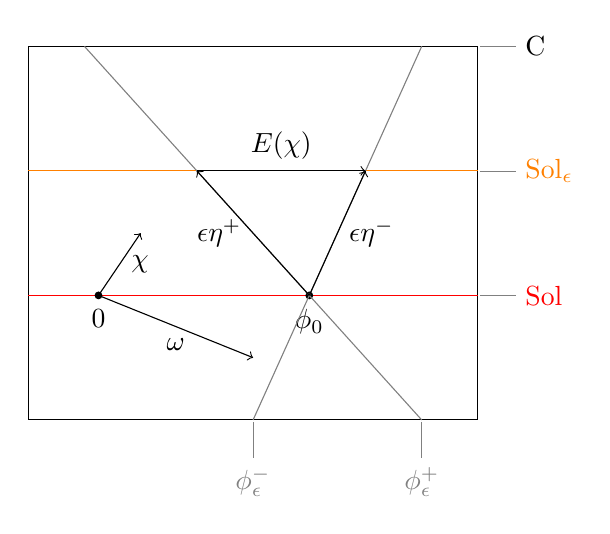
\begin{tikzpicture}
\begin{axis}[axis lines=none,clip=false]

	% Il riquadro di \Conf
	\addplot[color=black] coordinates {
		(8,6) (0,6) (0,0)(8,0)(8,6)
		}node [pos=1,pin={0:$\Conf$},inner sep=0pt] {};

	% la retta di \Sol
	\addplot[color=red] coordinates {
		(0,2)
		(8,2)
	}node [pos=1,pin={0:$\Sol$},inner sep=0pt] {};
	
	% Zero section
	\node[label={270:{$0$}},circle,fill,inner sep=1pt] at (axis cs:1.25,2) {};
	% Fixed Solution
	\node[label={270:{$\phi_0$}},circle,fill,inner sep=1pt] at (axis cs:5,2) {};

	% La curva di \Sol_\epsilon
	\addplot[color=orange] coordinates {
	(0,4)(8,4)
	}node [pos=1,pin={0:$\Sol_\epsilon$},inner sep=0pt] {};

	%Variation
	\addplot[color=gray] coordinates {
		(1,6)
		(7,0)
	}node [pos=1,pin={270:$\phi_\epsilon^+$},inner sep=0pt] {};
	\addplot[color=gray] coordinates {
		(7,6)
		(4,0)
	}node [pos=1,pin={270:$\phi_\epsilon^-$},inner sep=0pt] {};
	
	%Perturbation
	\addplot[->] coordinates
           {(5,2) (3,4)}node [pos=0.5,label={180:$\epsilon \eta^+$},inner sep=0pt] {};
	\addplot[->] coordinates
           {(5,2) (6,4)}node [pos=0.5,label={0:$\epsilon \eta^-$},inner sep=0pt] {};

	%AdvancedMinusRetarded
	\addplot[->] coordinates
           {(3,4) (6,4)}node [pos=0.5,label={90:$E (\chi)$},inner sep=0pt] {};
           
	%LagrangianDensities
	\addplot[->] coordinates
           {(1.25,2) (4,1)}node [pos=0.5,label={270:$\omega$},inner sep=0pt] {};	
	\addplot[->] coordinates
           {(1.25,2) (2,3)}node [pos=0.5,label={0:$\chi$},inner sep=0pt] {};		
	
	

\end{axis}
\end{tikzpicture}


%\/\/\/\/\/\/\/\/\/\/\/\/\/\/\/\/\/\/\/\/\/\/\/\/\/\/\/\/\/\/\/\/\/\/\/\/\/\/\/\/\/\/\/\/\/\/\/\/\/\/\/\/\/\/\/\/\/\/\/\/\/\/\/\/\/\/
\end{document}

